\documentclass[conference]{IEEEtran}
\IEEEoverridecommandlockouts
% The preceding line is only needed to identify funding in the first footnote. If that is unneeded, please comment it out.
\usepackage{cite}
\usepackage{amsmath,amssymb,amsfonts}
\usepackage{algorithmic}
\usepackage{graphicx}
\usepackage{textcomp}
\usepackage{xcolor}
\def\BibTeX{{\rm B\kern-.05em{\sc i\kern-.025em b}\kern-.08em
    T\kern-.1667em\lower.7ex\hbox{E}\kern-.125emX}}
\begin{document}

\title{DS 340W Week Six Report\\
%{\footnotesize \textsuperscript{*}Note: Sub-titles are not captured in Xplore and
% should not be used}
%\thanks{Identify applicable funding agency here. If none, delete this.}
{\footnotesize Group 10}
}

\author{\IEEEauthorblockN{Zheng Zhang}
\IEEEauthorblockA{\textit{Department of Statistics, Eberly College of Science} \\
\textit{Pennsylvania State University}}
\and
\IEEEauthorblockN{Madison Novak}
\IEEEauthorblockA{\textit{Department of EECS, College of Engineering} \\
\textit{Pennsylvania State University}}
}

\maketitle

% \begin{abstract}
% This document is a model and instructions for \LaTeX.
% This and the IEEEtran.cls file define the components of your paper [title, text, heads, etc.]. *CRITICAL: Do Not Use Symbols, Special Characters, Footnotes, 
% or Math in Paper Title or Abstract.
% \end{abstract}

% \begin{IEEEkeywords}
% component, formatting, style, styling, insert
% \end{IEEEkeywords}

\section{Introduction}
The Encyclopedia of DNA Elements (ENCODE) Consortium is organizing a challenge to accurately impute biochemical data associated with functional genomics elements in a variety of cell types. This paper will discuss Group 10s Week 6 project mark where we will discuss the updates pertaining to the challenge. This paper will be broken up into three sections: Data Pre-Processing, Evaluation Metrics Pipeline, and Exploratory Data Analysis. 
% \begin{figure}[htbp]
% \centerline{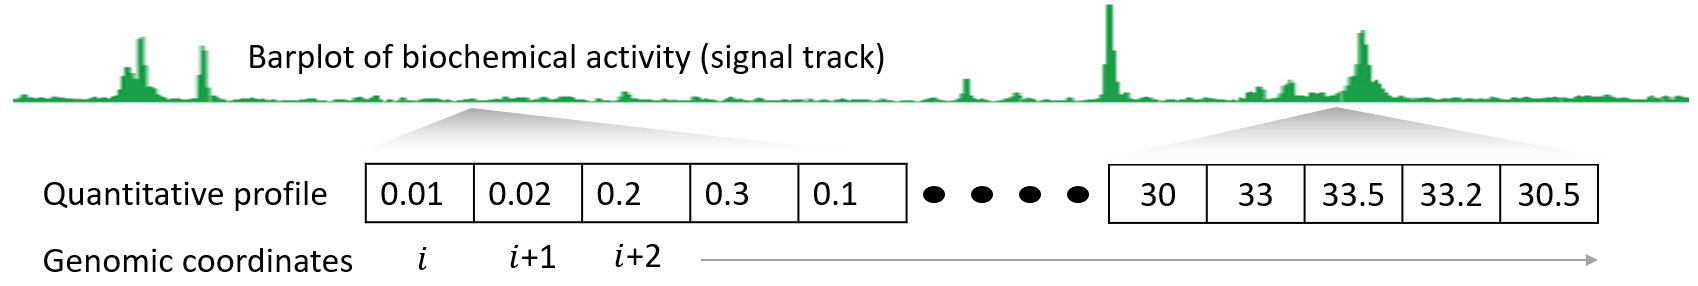
\includegraphics[width=0.50\textwidth]{img/Fig1-SignalTrack.png}}
% \caption{Example Data (Signal Track)}
% \label{fig}
% \end{figure}

\section{Data Pre-processing}
In order to obtain the massive data-sets from the Synapse organization website, we first installed the synapse python client on our local XSEDE cluster. We wrote the shell-script for automatically downloading all of the data to the allocation. The original thought was to treat the shell script as a job to submit, however, the job failed instantly after the script tried to connect to the internet. Therefore, our solution is to directly watch the script running on our local cluster to download the data. 

Since the original data-sets we downloaded are compressed files in .bigwig format, we have to convert them to the human-and-machine readable format such as .wig and .txt. In this case, we found out that the linux binary package for handling the bioinformatics data-sets developed by University of California - Santa Cruz (UCSC) is exceptionally useful and efficient. We installed those binary files and wrote a driver script to submit the data-processing jobs in parallel. Though we've made all of the scripts as parallel as possible, the size of the data-sets is still a key-issue in maintaining the running time. 

\section{Evaluation Metrics Pipeline}
For setting up a proper pipeline for the Evaluation Metrics we wanted to follow the guide for the Scoring/Ranking given by the ENCODE challenge github. Through Linux we were able to install Anaconda in order to be able to use the python data science packages like numpy and Sci-kit-Learn. Then we will take a possible submission and validate it through the given python file of validate.py. Since these files are very large we will be converting the files of "ENCFF622DXZ" and "ENCFF074VQD" from the ENCODE portal and converting them to a numpy array. The reason we will be doing this is because not only will it speed up the process but we will also be able to score multiple submissions at once through our bigWig. It is up to the groups if they want to score with or without variance but we find it to be beneficial to score with variance in mind. After all of our submissions are scored through the python libraries we will be creating a score database which will allow us to access all of our submission in one place. This will be convenient in seeing which models worked best and why.


\section{Exploratory Data Analysis}
For the Exploratory Data Analysis, we wanted to make sure that we investigated the data for each of the mark/cell types. Therefore we closely investigated visualizing the number of validation data associated with each mark type. For this problem we found that there were a multiple values of 0 so we decided to remove those 0 values for visualization. 
\begin{figure}[htp]
    \centering
    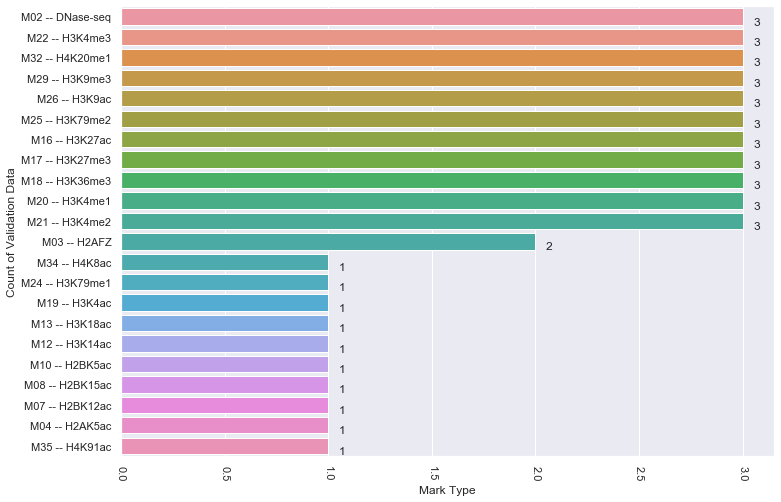
\includegraphics[width=6cm]{output_17_1.png}
    \caption{Visualizing data associated with each mark type}
    \label{fig:Mark Type}
\end{figure}

Through our research and analysis we have found that most of the data is heavily skewed to the right. This can be seen best by the sample distribution plot like the one we have shown in this paper. It is important to note that even though most of the data is skewed to the right, it does provide us with much information for further our knowledge on the characteristics of the data set. 

\begin{figure}
    \centering
    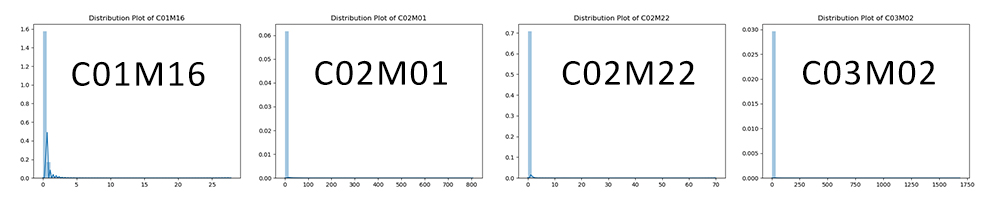
\includegraphics[width=8cm]{img/dist.jpg}
    \caption{Sample Training/Validation Data Distribution}
    \label{fig:my_label}
\end{figure}

\end{document}
